\chapter{Verbal Fluency PET data \label{Chap:data:pet}}

\section{Introduction}

These data come from a 5 subject PET study of a verbal fluency with two alternating word generation conditions: A (baseline) - word shadowing; B - (activation) - paced orthographic word generation. This involved responding with a word beginning with an aurally presented letter. Both conditions were identically paced at 1 word every 2 seconds. The presentation order alternated between AB and BA across subjects as shown in Table~\ref{conditions}.

\begin{table}[h]
\begin{center}
\begin{tabular}{ccccccccccccc}
  Scan: & 1 & 2 & 3 & 4 & 5 & 6 & 7 & 8 & 9 & 10 & 11 & 12 \\  \hline
  Subject 1& A & B & A & B& A & B& A & B& A & B& A & B \\
  Subject 2& B & A & B& A & B& A & B& A & B& A & B & A \\
  Subject 3& A & B & A & B& A & B& A & B& A & B& A & B \\
  Subject 4& B & A & B& A & B& A & B& A & B& A & B & A \\
  Subject 5& A & B & A & B& A & B& A & B& A & B& A & B \\ \hline
\end{tabular}
\end{center}
\caption{\em \textbf{Conditions for PET data:} (A) word shadowing and (B) word generation. \label{conditions}}
\end{table}

The files are named \verb!./p#/snrp#_##.{img,hdr}! and are SPM compatible (Analyze) images following realignment, normalization and smoothing with a 16mm isotropic Gaussian kernel with \verb!#! indicating the subject and \verb!##! the scan. The data set is available from the SPM website\footnote{Verbal Fluency PET dataset: \url{http://www.fil.ion.ucl.ac.uk/spm/data/fluency/}}.

To analyse the data, first create a new directory \texttt{DIR}, eg. \texttt{c:$\backslash$data$\backslash$pet}, in which to place the results of your analysis. Then create 4 subdirectories (i) \texttt{single}, (ii) \texttt{subject-condition}, (iii) \texttt{subject-time} and (iv) \texttt{multiple}.
As the analysis proceeds these directories will be filled with job-specification files, design matrices and estimated models.

\section{Single subject}

Firstly, we will analyse the data from a single subject. This can be implemented as follows.
\begin{itemize}
\item{Start up \matlab\ and type \texttt{spm pet} at the prompt}
\item{Press the ``Basic models'' button.}
\item{In `Factorial design specification', choose the `Flexible Factorial' design.}
\item{Highlight `Factors' and create a new Factor and enter 'Word' for the name.}
\item{Then, under 'Specify Subject or all Scans and Factors', highlight `Subjects' and create a new subject.}
\item{Highlight `Scans', select `Specify Files' and use the SPM file selector to choose the 12 images for that subject. This can be most easily achieved by specifying `.*snrp1.*' as a filter in the file selector.}
\item{Under `Conditions' enter the vector [1 2 1 2 1 2 1 2 1 2 1 2].}
\item{Under `Main effects and interactions', create a single main effect with factor number equal to 1}
\item{Under `Covariates', create a new covariate and enter `Time' for `Name' and the vector `1:12'.}
\item{Under `Global calculation' choose `Mean'}
\item{Under Global normalisation and Normalisation, choose `Proportional' scaling.\footnote{Normalisation using ANCOVA is advised for multi-subject studies unless differences in global flow are large eg. due to variability in injected tracer dose. Because ANCOVA uses one degree of freedom for each subject/group, proportional scaling may be preferable for single-subject studies.}}
\item{Under Global normalisation and Overall grand mean scaling, select YES.}
\item{Highlight Directory, Specify files and select the subdirectory `single', to place the design matrix in.}
\item{Save the job file as eg. \texttt{DIR/single\_design.mat}.}
\item{Press the \texttt{Run} button (green arrow).}
\end{itemize}
SPM will then show you the design matrix shown in Figure~\ref{single_design}. This design is encoded in the \texttt{SPM.mat} file that is written to the output directory.
\begin{figure}
\begin{center}
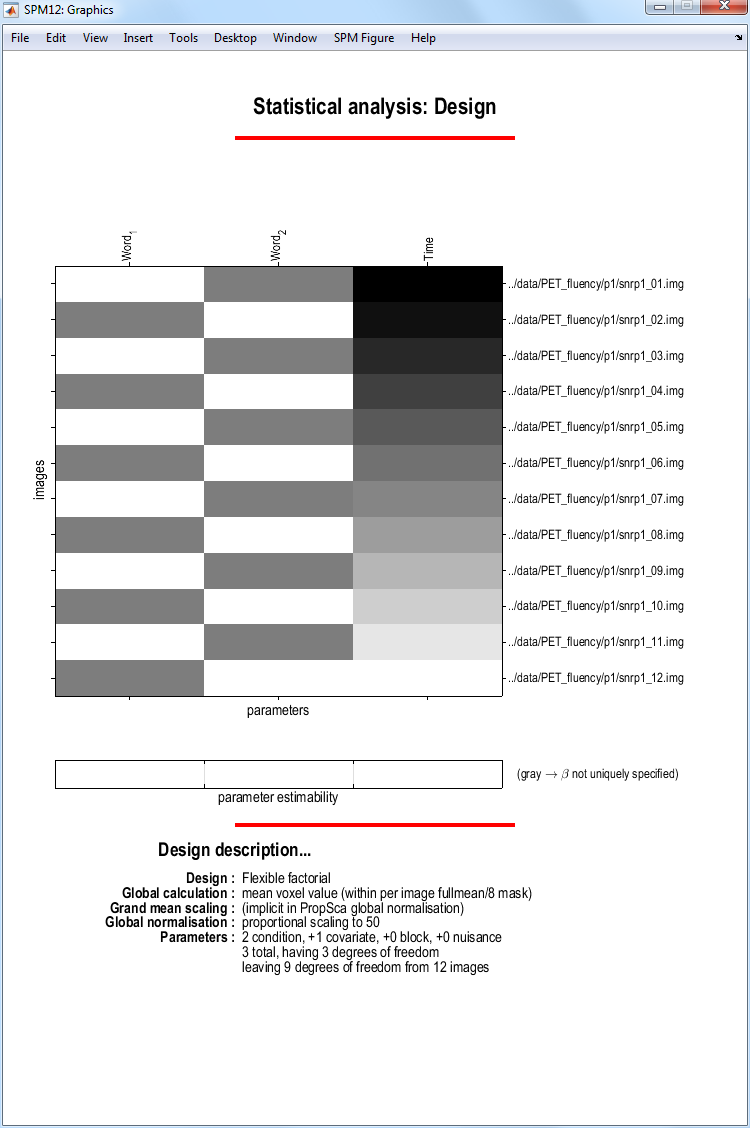
\includegraphics[width=100mm]{pet/single_design}
\caption{\em Design matrix for single-subject data. The first two columns model responses to word shadowing and word generation. The third column models time-varying responses. \label{single_design}}
\end{center}
\end{figure}
Then press `Estimate' and select the \texttt{SPM.mat} file just created. SPM will now estimate the parameters, that is, the size of the population effect at each voxel.
\begin{itemize}
\item{Now press the 'Results' button.}
\item{Select the \texttt{SPM.mat} file.}
\item{In the contrast manager press 'Define new contrast' (select T). Enter [-1 1] in the contrast section and enter 'activation' as a 'name'.}
\item{Press the 'submit' button. Press OK.}
\item{Now press the 'Done' button.}
\item{Mask with other contrast(s) [No]}
\item{p value adjustment to control [FWE]}
\item{Family-wise p-value [0.05]}
\item{Extent threshold {voxels} [0]}
\end{itemize}
You should see a blank MIP as, sadly, we rarely have enough sensitivity to find activations in single subject PET data. This is why we scan multiple subjects.

\section{Multiple subjects}

The data set can be analysed in several ways  which are discussed in \cite{stefan_hbf2}.

\subsection{Subject and Condition design}

First we set up a design that allows us to test for the main effects of `Subject' and `Condition'. The design can be set-up as follows.
\begin{itemize}
\item{Start up \matlab\ and type \texttt{spm pet} at the prompt}
\item{Press the `Basic Models' button.}
\item{In `Factorial design specification', under `Design', choose the `Flexible Factorial' design.}
\item{Highlight `Factors' and create a new Factor.}
\item{Enter 'Subject' for the name and select 'Equal' under `Variance'.}
\item{Then create another factor and call it `Word'}
\item{Then, under 'Specify Subject or all Scans and Factors', highlight `Subjects' and create a 5 new subjects.}
\item{For the first subject, highlight `Scans', select `Specify Files' and use the SPM file selector to choose the 12 images for the first subject. This can be most easily achieved by specifying \texttt{.*snrp1.*} as a filter in the file selector and then using a right click to `select all'.}
\item{Under `Conditions' enter the vector [1 2 1 2 1 2 1 2 1 2 1 2].}
\item{Repeat the specification of scans and conditions for each of the four other subjects, remembering that the order of conditions has been balanced across the group (see Table~\ref{conditions}).}
\item{Under `Main effects and interactions', create two main effects, the first with factor number 1 (ie. Subject) and the second with factor number 2 (ie. Word).}
\item{Under Masking, select `Relative' for `Threshold Masking' and accept the default value of 0.8. Voxels with mean value less than 0.8 of the mean are deemed extra-cranial and will be excluded from the analysis.}
\item{Under `Global calculation' choose `Mean'}
\item{Under, Global normalisation, and Normalisation, select 'ANCOVA'.}
\item{Highlight Directory, Specify files and select the subdirectory `subject-condition', to place the design matrix in.}
\item{Save the job file as eg. \texttt{DIR/sc\_design.mat}.}
\item{Press the \texttt{Run} button.}
\end{itemize}
SPM will then show you the design matrix shown in Figure~\ref{sc_design}. This design is encoded in the \texttt{SPM.mat} file that is written to the output directory.
\begin{figure}
\begin{center}
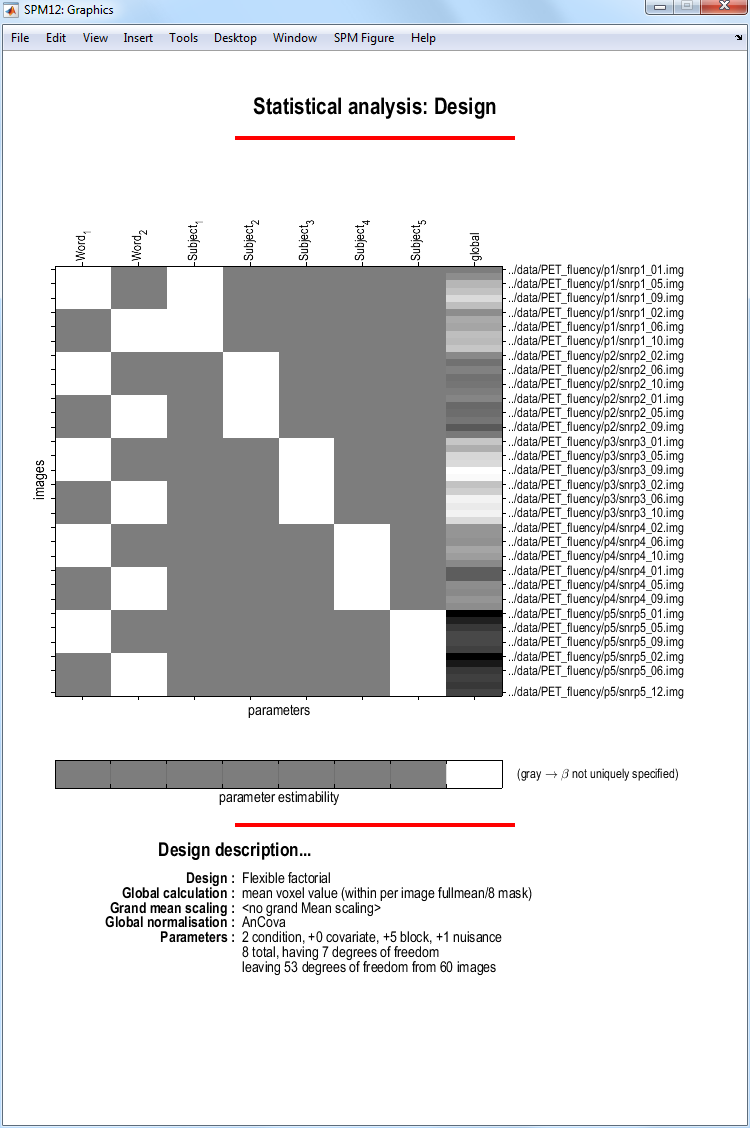
\includegraphics[width=100mm]{pet/sc_design}
\caption{\em Subjects and Conditions design for multiple-subject data. The first five columns model effect and the next two columns model condition effects. The last colum models global effects (ANCOVA).  \label{sc_design}}
\end{center}
\end{figure}

\subsection{Subject and Time design}

We now set up a design that allows us to test for the effects of Time (ie. scan number) and Subject. If you have already specified the Subject and Conditions design, then you can set up the Subject and Time design by editing the \texttt{sc\_design.mat} file (and just changing the name of the second factor, Conditions vector and output directory - see below). Otherwise, the design can be set-up as follows.
\begin{itemize}
\item{Start up \matlab\ and type \texttt{spm pet} at the prompt}
\item{Press the `Basic Models' button.}
\item{In `Factorial design specification', under `Design', choose the `Flexible Factorial' design.}
\item{Highlight `Factors' and create a new Factor.}
\item{Enter 'Subject' for the name and select 'Equal' under `Variance'.}
\item{Then create another factor and call it `Time'. This factor extends over time for each subject.}
\item{Then, under 'Specify Subject or all Scans and Factors', highlight `Subjects' and create a 5 new subjects.}
\item{For the first subject, highlight `Scans', select `Specify Files' and use the SPM file selector to choose the 12 images for the first subject. This can be most easily achieved by specifying \texttt{.*snrp1.*} as a filter in the file selector and then using a right click to `select all'.}
\item{Under `Conditions' enter the vector [1:12].}
\item{Repeat the specification of scans and conditions for each of the four other subjects.}
\item{Under `Main effects and interactions', create two main effects, the first with factor number 1 (ie. Subject) and the second with factor number 2 (ie. Time).}
\item{Under Masking, select `Relative' for `Threshold Masking' and accept the default value of 0.8. Voxels with mean value less than 0.8 of the mean are deemed extra-cranial and will be excluded from the analysis.}
\item{Under `Global calculation' choose `Mean'}
\item{Under, Global normalisation, and Normalisation, select 'ANCOVA'.}
\item{Highlight Directory, Specify files and select the subdirectory `subject-condition', to place the design matrix in.}
\item{Save the job file as eg. \texttt{DIR/st\_design.mat}.}
\item{Press the \texttt{Run} button.}
\end{itemize}
SPM will then show you the design matrix shown in Figure~\ref{st_design}. This design is encoded in the \texttt{SPM.mat} file that is written to the output directory.
\begin{figure}
\begin{center}
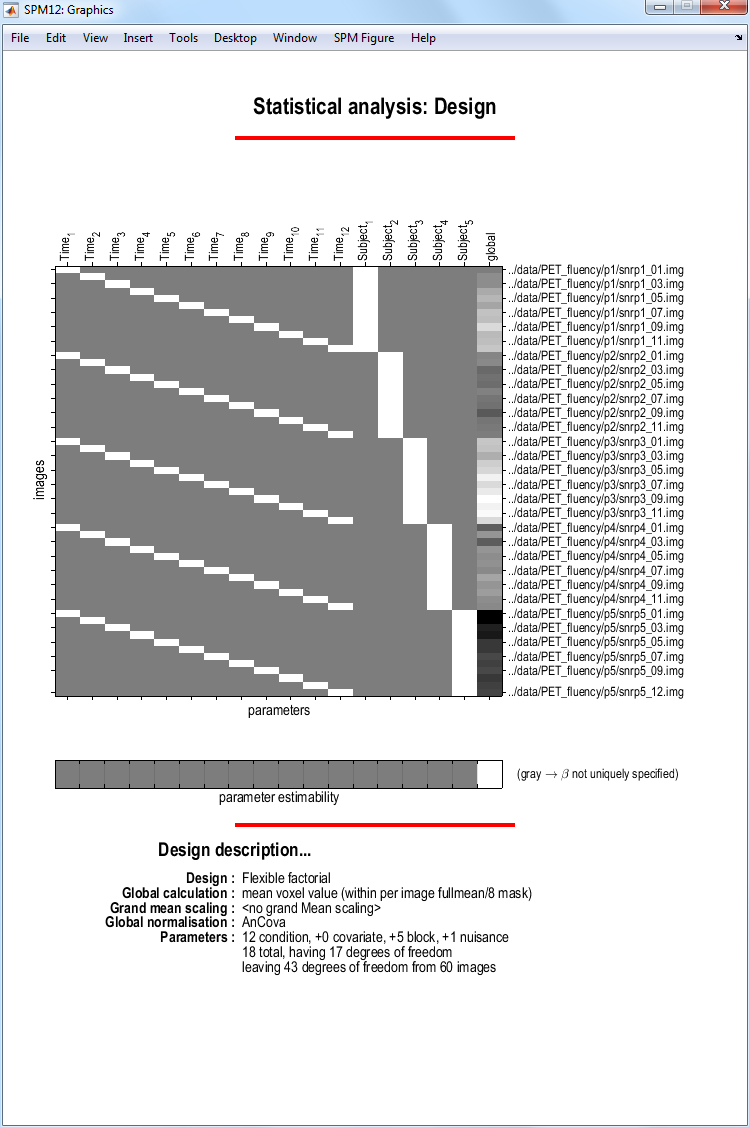
\includegraphics[width=100mm]{pet/st_design}
\caption{\em Subjects and Time design for multiple-subject data. The first five columns model subjects effects and the next 12 model time effects. The last column models global effects (ANCOVA).  \label{st_design}}
\end{center}
\end{figure}

\subsection{Subject by Condition design}

This design models the interacts between `Subject' and `Condition'. It allows effects to be assessed separately for each subject. It will also allow us to implement
a conjunction analysis over subjects.

If you have already specified the Subject and Conditions or Subject and Time designs then this design can be more easily specified by editing the \texttt{sc\_design.mat} or \texttt{st\_design.mat} files (and changing the name of the second factor, removing main effects, adding the interaction term and specifying a new output directory - see below). Otherwise, the design can be set-up as follows.
\begin{itemize}
\item{Start up \matlab and type \texttt{spm pet} at the prompt}
\item{Press the ``Basic Models'' button.}
\item{In `Factorial design specification', under `Design', choose the `Flexible Factorial' design.}
\item{Highlight `Factors' and create a new Factor.}
\item{Enter 'Subject' for the name and select 'Yes' under ANCOVA, as we will be implementing ANCOVA-by-subject. Select 'Equal' under `Variance'.}
\item{Then create another factor and call it `Word'}
\item{Then, under 'Specify Subject or all Scans and Factors', highlight `Subjects' and create a 5 new subjects.}
\item{For the first subject, highlight `Scans', select `Specify Files' and use the SPM file selector to choose the 12 images for the first subject. This can be most easily achieved by specifying `.*snrp1.*' as a filter in the file selector and then using a right click to `select all'.}
\item{Under `Conditions' enter the vector [1 2 1 2 1 2 1 2 1 2 1 2].}
\item{Repeat the specification of scans and conditions for each of the four other subjects, remembering that the order of conditions has been balanced across the group (see Table~\ref{conditions}).}
\item{Under `Main effects and interactions', create an interaction with factor numbers equal to [1 2]. This will create a block in the design matrix that models interactions between the factors `Subject' and `Word'.}
\item{Under Masking, select `Relative' for `Threshold Masking' and accept the default value of 0.8. Voxels with mean value less than 0.8 of the mean are deemed extra-cranial and will be excluded from the analysis.}
\item{Under `Global calculation' choose `Mean'}
\item{Highlight Directory, Specify files and select the subdirectory \texttt{multiple}, to place the design matrix in.}
\item{Save the job file as eg. \texttt{DIR/multi\_design.mat}}.
\item{Press the \texttt{Run} button.}
\end{itemize}
SPM will then show you the design matrix shown in Figure~\ref{multi_design}. This design is encoded in the `SPM.mat' file that is written to the output directory.
\begin{figure}
\begin{center}
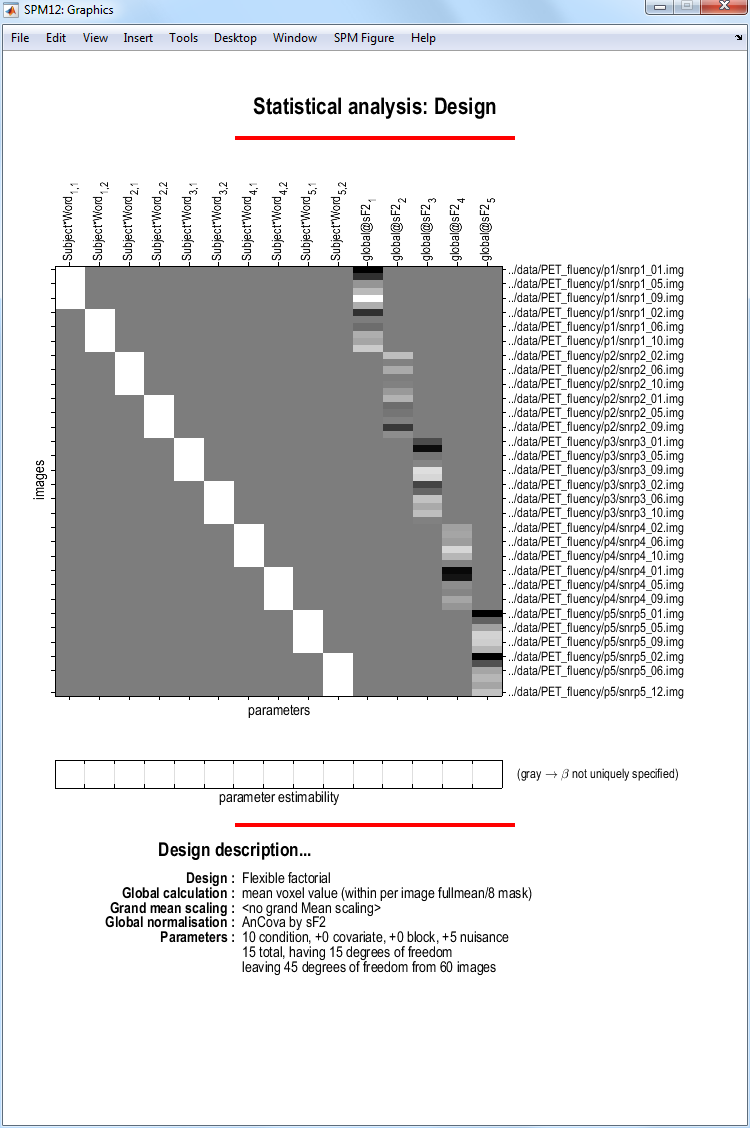
\includegraphics[width=100mm]{pet/multi_design}
\caption{\em Subject by Condition design for multiple-subject data. The first ten columns model interactions between `Subject' and `Word'. The last five columns model out global effects for each subject. Inclusion of these last five regressors implements
a so-called `ANCOVA-by-subject' normalisation. \label{multi_design}}
\end{center}
\end{figure}
Then press `Estimate' and select the \texttt{SPM.mat} file just created. SPM will now estimate the parameters, that is, the size of the effect at each voxel. The rest of this chapter pursues the `Subject-by-Condition' design.

\subsection{Contrast manager}

We can then examine relative activations, that is, regions which respond more strongly during word generation than word shadowing, for each subject. For subject 2:
\begin{itemize}
\item{Press the 'Results' button.}
\item{Select the \texttt{SPM.mat} file.}
\item{In the contrast manager press 'Define new contrast' (select T)}
\item{Specify e.g. \verb!Subject 2: Gen > Shad! (name) and '0 0 -1 1' (contrast).}
\item{Press the 'submit' button. Press OK.}
\item{Now press the 'Done' button.}
\item{Mask with other contrast(s) [No]}
\item{p value adjustment to control [FWE]}
\item{Family-wise p-value [0.05]}
\item{Extent threshold {voxels} [0]}
\end{itemize}
This should produce the contrast in Figure~\ref{subject2}. As shown, SPM will automatically pad '0 0 -1 1' with zeros
at the end.
\begin{figure}
\begin{center}
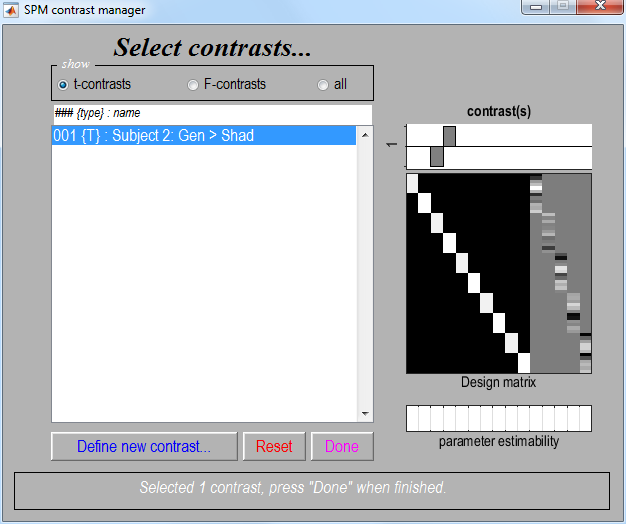
\includegraphics[width=100mm]{pet/subject2}
\caption{\em Activation contrast for subject 2. Note that the block of the design matrix encoding the experimental conditions is now coloured differently. This is because we have allowed the variance of responses over subjects to be different between word shadowing and generation conditions. This `nonsphericity' affects parameter estimation in a way that is implemented in SPM by first `colouring' the design matrix and then implementing ordinary least squares. This, in no way however, affects interpretation of effects.  \label{subject2}}
\end{center}
\end{figure}
To examine group effects:
\begin{itemize}
\item{Press the 'Results' button.}
\item{Select the SPM.mat file.}
\item{In the contrast manager press 'Define new contrast' (select T)}
\item{Specify e.g. \verb!All: Gen > Shad! (name) and  '-1 1 -1 1 -1 1 -1 1 -1 1' and select it (press 'Done') (contrast).}
\item{Mask with other contrast(s) [No]}
\item{Title for comparison [activation]}
\item{p value adjustment to control [FWE]}
\item{Family-wise p-value [0.05]}
\item{Extent threshold {voxels} [0]}
\end{itemize}
Before looking at the results we describe the
masking and thresholding options in more detail.

\subsection{Masking and thresholds}

Masking implies selecting voxels specified by other contrasts. If 'yes', SPM will prompt for (one or more) masking contrasts, the significance level of the mask (default p = 0.05 uncorrected), and will ask whether an inclusive or exclusive mask should be used. Exclusive will remove all voxels which reach the default level of significance in the masking contrast, inclusive will remove all voxels which do not reach the default level of significance in the masking contrast. Masking does not affect p-values of the 'target' contrast.

Selecting a height threshold for examine results uses either a threshold corrected for multiple comparisons ('yes'), or uncorrected ('no'). The latter will produce many false positives (FPs) in the SPM. On average, the number of false positives will be equal to the number of voxels in the volume times the
p-value (eg. $50,000 \times 0.001 = 50$). If you correct for multiple comparisons, however, then
there will typically be only one FP {\em anywhere} in 20
SPMs. Correcting for multiple comparisons is the recommended
option.

Specifying an extent threshold $x$ tells SPM not to plot clusters containing fewer than $x$ voxels. The default, $x=0$ allows single voxel activations to be displayed.

\subsection{MIPs and results tables}

The above contrast specifications should configure the contrast manager to appear as in Figure~\ref{all} and will configure SPM's graphics window to look like Figure~\ref{all_results}.
\begin{figure}
\begin{center}
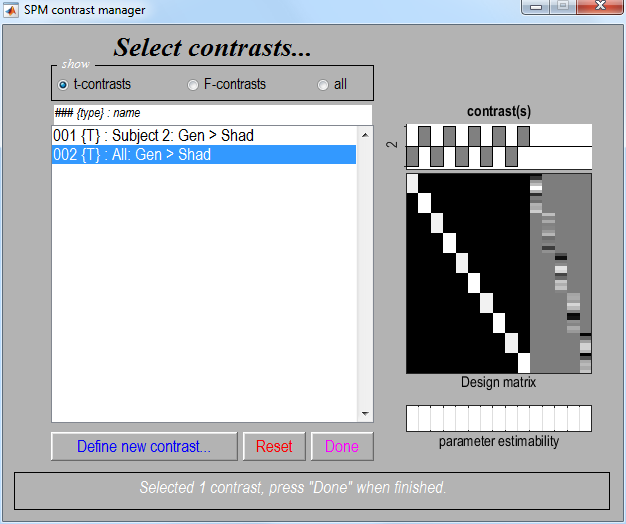
\includegraphics[width=100mm]{pet/all}
\caption{\em Activation contrast for all subjects.  \label{all}}
\end{center}
\end{figure}
\begin{figure}
\begin{center}
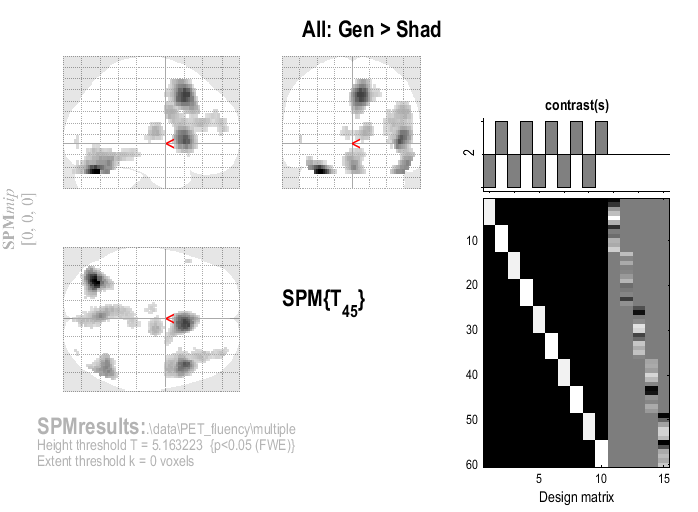
\includegraphics[width=100mm]{pet/all_results}
\caption{\em SPMs graphics window displays (Left) a maximum intensity projection (MIP) on a glass brain in three orthogonal planes. The MIP is surfable: right-clicking in the MIP will activate a pulldown menu, left-clicking  on the red cursor will allow it to be dragged to a new position, (Right)  the design matrix (showing the selected contrast). The design matrix is also surfable: right-clicking will show parameter names, left-clicking will show design matrix values for each scan. \label{all_results}}
\end{center}
\end{figure}

SPM will also produce a number of files: images containing weighted parameter estimates are saved as \verb!con_0002.hdr/img!, \verb!con_0003.hdr/img!, etc. in the output directory. Images of T-statistics are saved as \verb!spmT_0002.hdr/img!, \verb!spmT_0003.hdr/img!, etc., also in the output directory. A number of
further options are available from SPM Interactive window shown in Figure~\ref{interactive}.
\begin{figure}
\begin{center}
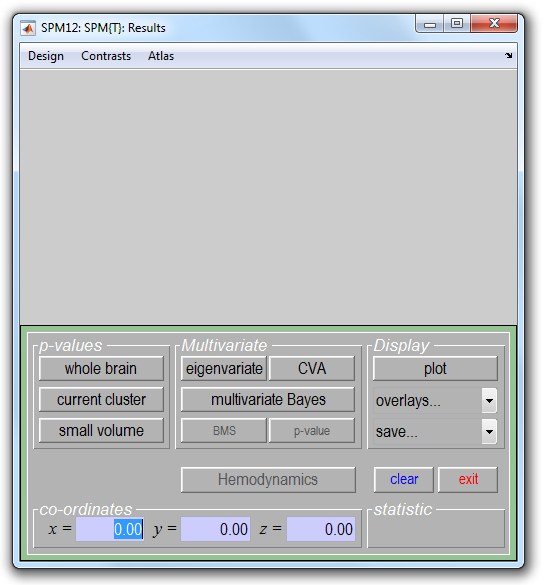
\includegraphics[width=100mm]{pet/interactive}
\caption{\em SPM's interactive window.  \label{interactive}}
\end{center}
\end{figure}

In the SPM Interactive window (lower left panel) a button box appears with various options for displaying statistical results (p-values panel) and creating plots/overlays (visualisation panel). Clicking 'Design' (upper left) will activate a pulldown menu as in the 'Explore design' option. To get a summary of local maxima, press 'volume'. This will produce the table shown in Figure~\ref{table}.
\begin{figure}
\begin{center}
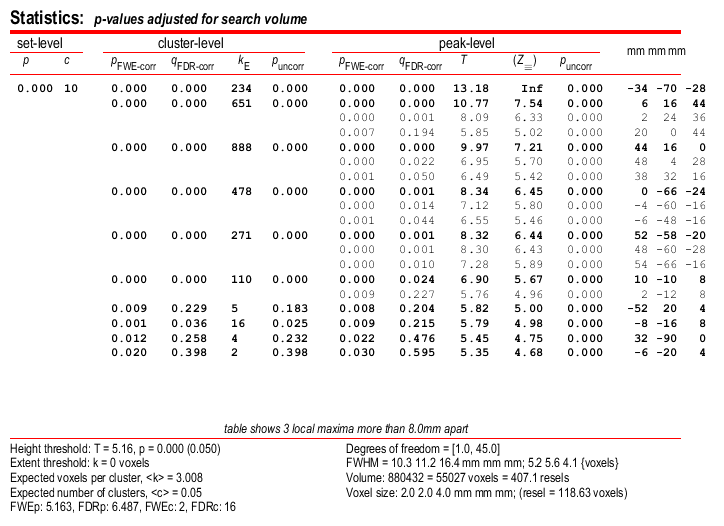
\includegraphics[width=100mm]{pet/table}
\caption{\em SPM results table. This appears below the MIP, shown in Figure~\ref{all_results}, in the graphics window. \label{table}}
\end{center}
\end{figure}
As in the previous example, this will list all clusters above the chosen level of significance as well as separate ($>$8mm apart) maxima within a cluster, with details of significance thresholds and search volume underneath. The columns show, from right to left:
\begin{itemize}
\item{\textbf{x, y, z (mm):} coordinates in Talairach space for each maximum.}
\item{\textbf{peak-level:} the chance (p) of finding (under the null hypothesis) a peak with this or a greater height (T- or Z-statistic), corrected / uncorrected for search volume.}
\item{\textbf{cluster-level:} the chance (p) of finding a cluster with this or a greater size (ke), corrected / uncorrected for search volume.}
\item{\textbf{set-level:} the chance (p) of finding this or a greater number of clusters (c) in the search volume.}
\end{itemize}
Its also worth noting that
\begin{itemize}
\item{The table is surfable: clicking a row of cluster coordinates will move the pointer in the MIP to that cluster, clicking other numbers will display the exact value in the Matlab window (e.g. 0.000 = 6.1971e-07).}
\item{To inspect a specific cluster, either move the cursor in the MIP (by L-clicking \& dragging the cursor, or R-clicking the MIP background which will activate a pulldown menu).}
\item{Alternatively, click the cluster coordinates in the volume table, or type the coordinates in the lower left windows of the SPM Interactive window.}
\end{itemize}
Selecting 'cluster' will show coordinates and voxel-level statistics for local maxima ($>$4mm apart) in the selected cluster. See Figure~\ref{cluster}. The table is also surfable.
\begin{figure}
\begin{center}
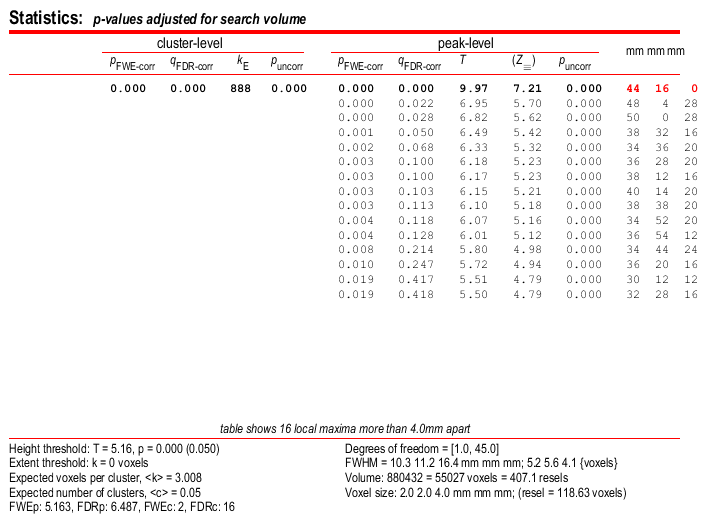
\includegraphics[width=100mm]{pet/cluster}
\caption{\em SPM results table for a single cluster with p-values corrected for the whole brain.  \label{cluster}}
\end{center}
\end{figure}
Both in the `volume' and `cluster' options, p-values are corrected for the entire search volume.

\subsection{Small volume correction}

If one has an a priori anatomical hypothesis, eg. in the present example Broca's area will likely be activated during word generation, one may use the small volume correction option. Press the ``small volume'' button in SPM Interactive (bottom left) window and select a suitable region, e.g., a 30mm sphere with its centre at 44 16 0.
The region can also be defined using mask images derived from previous imaging data. The corrected p-values will change,
as shown in Figure~\ref{svc}.
\begin{figure}
\begin{center}
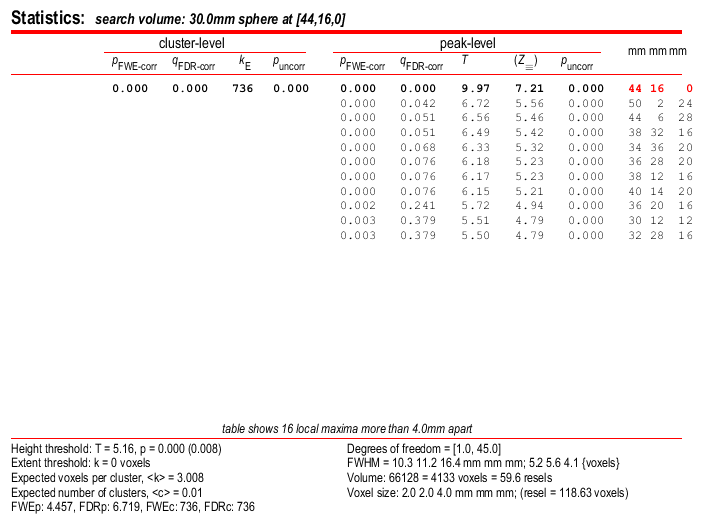
\includegraphics[width=100mm]{pet/svc}
\caption{\em SPM results table for a single cluster with p-values corrected using the Small Volume Correction (SVC) option. This used a 30mm sphere centred at 44 16 0. Note the reduced number of voxels in the search volume (bottom right text in Figure) and more significant p-values as compared to  Figure~\ref{cluster}. \label{svc}}
\end{center}
\end{figure}

\subsection{Extracting data from regions}

To extract a time course for data in this region of interest (this uses the SPM function \texttt{spm\_regions.m}):
\begin{itemize}
\item{Select ``eigenvariate'' from the ``Multivariate'' section in the Interactive window}
\item{Specify `Broca' for name of region and 0 for the VOI radius.}
\item{Select ('don't adjust')}
\end{itemize}
SPM displays a graph of the first eigenvariate of the data in or centered around the chosen voxel, as shown in Figure~\ref{voi}. It also lists the eigenvariate values $Y$ in the Matlab window.  Adjustment is with respect to the null space of a selected contrast.
This means that any effects not spanned by the chosen contrast
are removed from the data, before extraction. Adjustment can be
omitted by selecting `don't adjust', as above.

SPM extracts the eigenvariate values in a region, rather than the mean values, as the former is more robust to
heterogeneity of response within a cluster. The mean value can be thought of as a special case of the eigenvariate if the
corresponding eigenvector weights all voxels in a cluster
equally. Effectively, the
eigenvariate provides a weighted mean where atypical voxels are downweighted.

A file called \verb!VOI_regionname.mat! is created in the working directory containing Y and VOI details (in the data structure xY).

\begin{figure}
\begin{center}
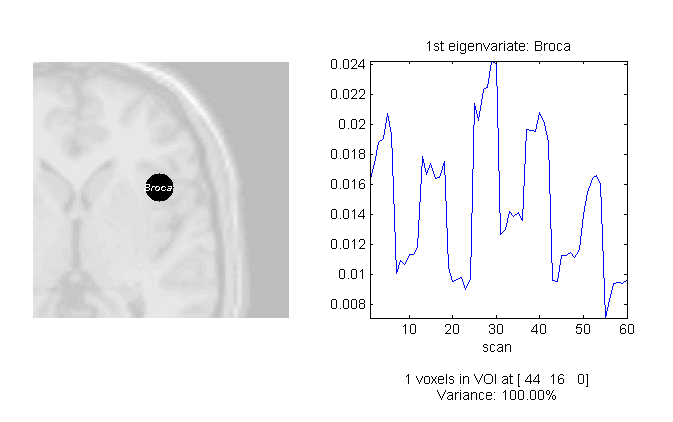
\includegraphics[width=100mm]{pet/voi}
\caption{\em Data extracted from a Volume of Interest (VOI). \label{voi}}
\end{center}
\end{figure}

\subsection{Inclusive Masking}

We have so far looked at the {\em average} effect over the five subjects in our group using the `All: Gen $>$ Shad' contrast.
To assess condition effects that are {\em common} to all subjects, one can either mask (inclusively) the `All: Gen $>$ Shad' contrast with the individual contrasts, or perform a conjunction analysis. Firstly we'll use the inclusive masking
approach.
\begin{itemize}
\item{Press the 'Results' button.}
\item{Select the SPM.mat file.}
\item{Select the \verb!All: Gen > Shad! contrast and press `Done'.}
\item{Mask with other contrast(s) [Yes]}
\item{Then hold down the [control] button whilst selecting all the individual contrasts. The contrast manager should then appear as in Figure~\ref{masked_con}.}
\item{Uncorrected mask p-value [0.05]}
\item{Nature of mask [inclusive]}
\item{p value adjustment to control [FWE]}
\item{Family-wise p-value [0.05]}
\item{Extent threshold {voxels} [0]}
\end{itemize}
This should produce the MIP and results table shown in Figure~\ref{masked_res}.
\begin{figure}
\begin{center}
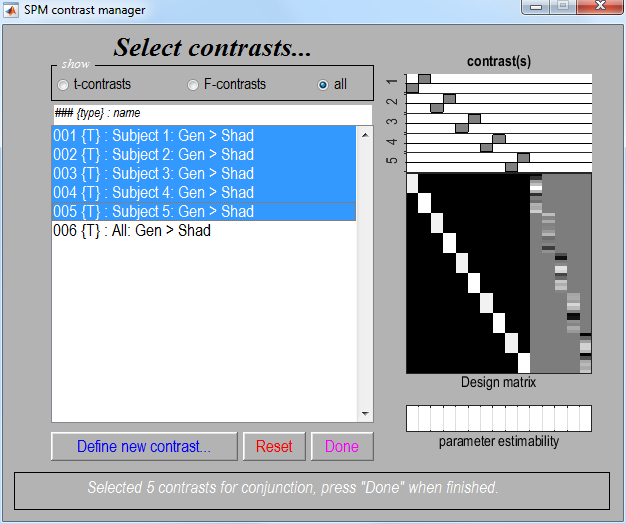
\includegraphics[width=100mm]{pet/masked_con}
\caption{\em SPM can produce maps based on multiple contrasts by holding down [control] whilst selecting contrasts. This can be used during masking and when making a conjunction inference. \label{masked_con}}
\end{center}
\end{figure}
\begin{figure}
\begin{center}
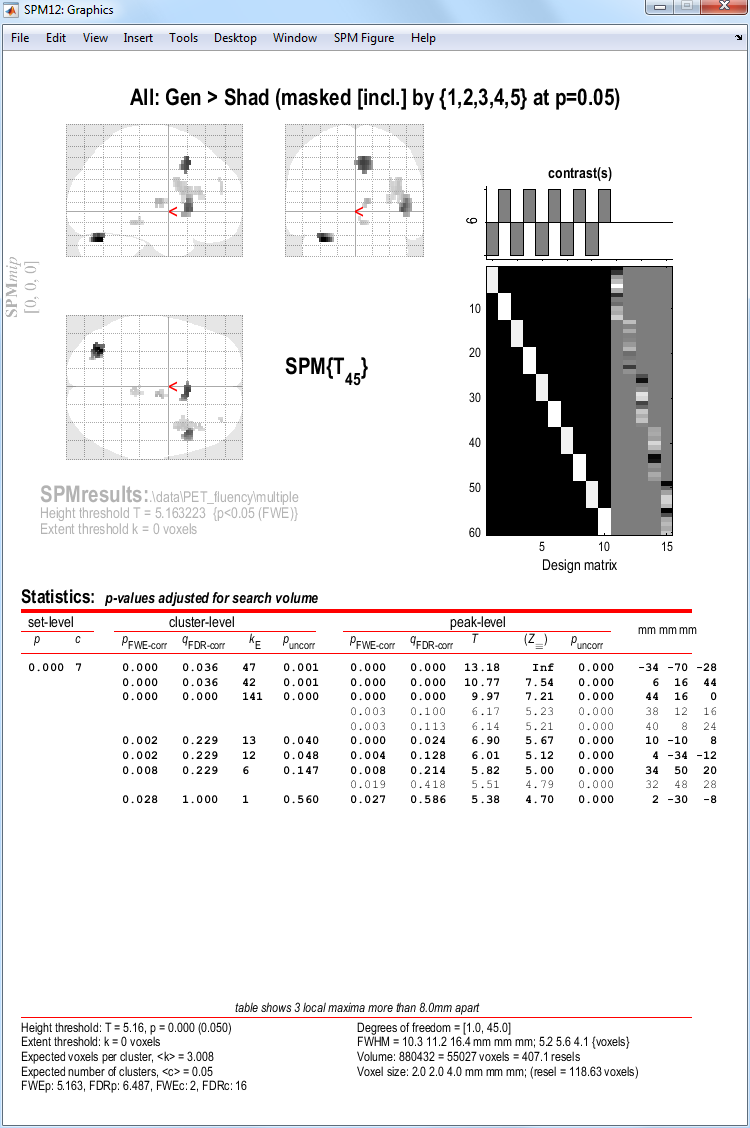
\includegraphics[width=100mm]{pet/masked_res}
\caption{\em The SPM shows results from the inclusive masking approach. It shows all voxels which are (a) significant at $p<0.05$ corrected across all subjects and (b) significant at $p<0.05$ uncorrected for each subject individually. \label{masked_res}}
\end{center}
\end{figure}

\subsection{Conjunctions}

To perform a conjunction approach across subjects:
\begin{itemize}
\item{Press the 'Results' button.}
\item{Select the SPM.mat file.}
\item{Then hold down the [control] button whilst selecting all the individual contrasts. The contrast manager should then appear as in Figure~\ref{masked_con} (except that, in the white text at the bottom, it should indicate that a conjunction will be performed).}
\item{Null hyp. to assess [Global]}
\item{Mask with other contrasts [No]}
\item{Title for comparison [accept the default]}
\item{p value adjustment to control [FWE]}
\item{Family-wise p-value [0.05]}
\item{Extent threshold {voxels} [0]}
\end{itemize}
SPM checks whether the contrasts are orthogonal and, if not,
makes them so. Contrasts are orthogonolized with respect to the first contrast specified.

SPM should produce the MIP and table of results shown in
Figure~\ref{conj}. The p-value (corrected or uncorrected) refers to the threshold of the conjunction. SPM will compute corresponding thresholds for individual contrasts. For uncorrected thresholds, the individual threshold will be $p^1/n$, where $p$ is the individual threshold and $n$ is
the number of contrasts in the conjunction.

Height, and not extent, is used to specify thresholding because the distributional approximations for the spatial extent of a conjunction SPM are not known (at present), so that inference based on spatial extent is precluded.

Although the MIP's of the masked group contrast and the conjunction are similar, for the conjunction an intersection SPM or 'minimum T-field' is computed.   This intersection is the same as thresholding a map of the minimum T-values. If the smallest T-value is above the specified threshold then all the T-values associated with the component SPMs are above threshold.

Conjunction SPMs are very useful for testing multiple hypotheses (each component hypothesis being specified by a contrast). In this example, we have chosen to use the
Global Null Hypothesis. The set of hypotheses tested jointly is that the first subject did not activate, the second subject did not activate and so on.

SPM also provides an option to use the Conjunction Null
hypothesis. This can be thought of as enabling an inference that subject 1 activated AND subject 2 activated AND subject 3... etc. For more discussion on this issue, see
\cite{karl_conj_revisit} and \cite{tom_valid}.

Gaussian field theory results are available for SPMs of minimum T- (or F-) statistics and therefore corrected p-values can be computed.  Note that the minimum T-values do not have the usual Student's T-distribution and small minimum T-values can be very significant.
\begin{figure}
\begin{center}
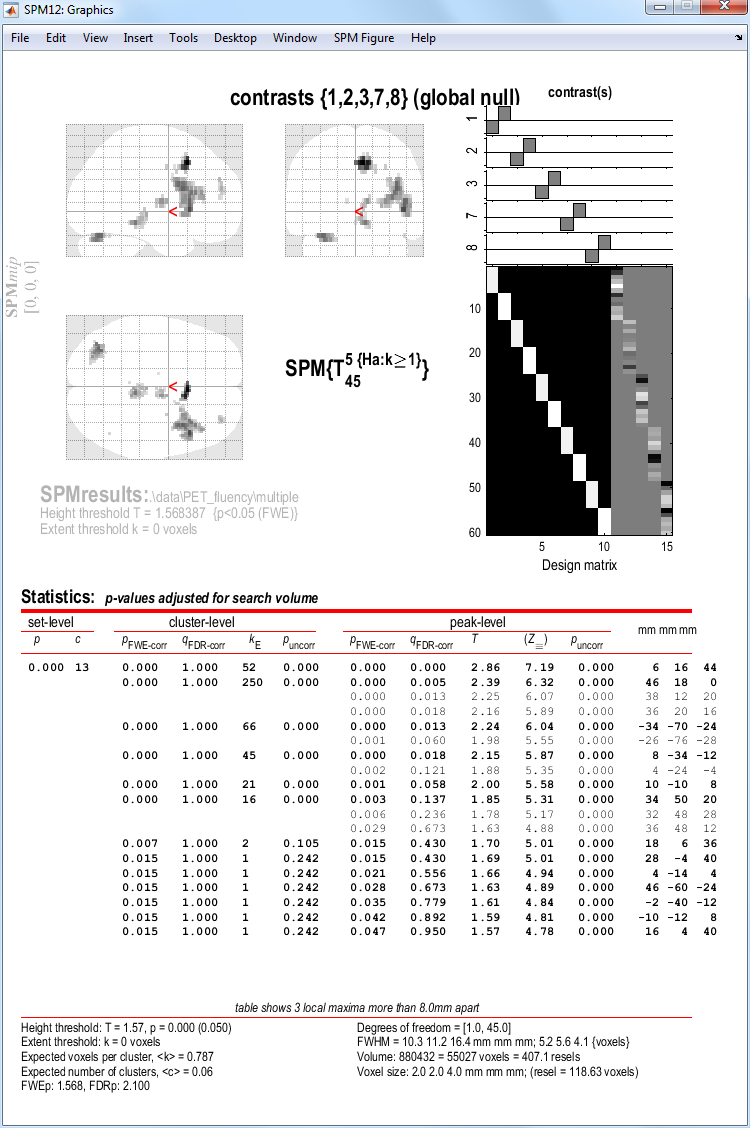
\includegraphics[width=100mm]{pet/conj}
\caption{\em Conjunction SPM. \label{conj}}
\end{center}
\end{figure}

